\begin{tikzpicture}
  \definecolor{lightGray}{HTML}{b3b3b3}
  \pgfmathsetmacro{\figureWidthPt}{\linewidth}

  \node (im) [inner sep=0pt] {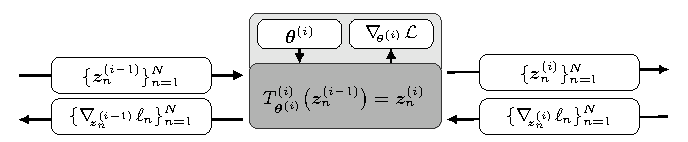
\includegraphics[width=\figureWidthPt pt]{../repos/backpack-paper/tex/paper/figs/backprop-modules/vanilla_backprop.pdf}};

  \newcommand{\relativeCoordinate}[2]{($(im.south west)!#1!(im.south east)+(im.south west)!#2!(im.north west)-(im.south west)$)}

  % bottom left
  \node [rectangle, fill=white, draw=none, inner sep=0pt, minimum height =
  0.04*\figureWidthPt pt, minimum width = 0.18*\figureWidthPt pt, anchor=center]
  at \relativeCoordinate{0.19}{0.18} {$\{ \grad{\vz_n^{(l-1)}}\ell_n \}_n$};

  % top left
  \node [rectangle, fill=white, draw=none, inner sep=0pt, minimum height =
  0.04*\figureWidthPt pt, minimum width = 0.18*\figureWidthPt pt, anchor=center]
  at \relativeCoordinate{0.19}{0.47} {$\{ \vz_n^{(l-1)}\}_n$};

  % bottom right
  \node [rectangle, fill=white, draw=none, inner sep=0pt, minimum height =
  0.04*\figureWidthPt pt, minimum width = 0.18*\figureWidthPt pt, anchor=center]
  at \relativeCoordinate{0.81}{0.18} {$\{ \grad{\vz_n^{(l)}}\ell_n \}_n$};

  % top right
  \node [rectangle, fill=white, draw=none, inner sep=0pt, minimum height =
  0.04*\figureWidthPt pt, minimum width = 0.18*\figureWidthPt pt, anchor=center]
  at \relativeCoordinate{0.81}{0.49} {$\{ \vz_n^{(l)}\}_n$};

  % center left
  \node [rectangle, fill=white, draw=none, inner sep=0pt, minimum height =
  0.035*\figureWidthPt pt, minimum width = 0.1*\figureWidthPt pt, anchor=center]
  at \relativeCoordinate{0.435}{0.76} {$\vtheta^{(l)}$};

  % center right
  \node [rectangle, fill=white, draw=none, inner sep=0pt, minimum height =
  0.035*\figureWidthPt pt, minimum width = 0.1*\figureWidthPt pt, anchor=center]
  at \relativeCoordinate{0.5685}{0.76} {$\grad{\vtheta^{(l)}}\gL$};

  % module
  \node [rectangle, fill=lightGray, draw=none, inner sep=0pt, minimum height =
  0.07*\figureWidthPt pt, minimum width = 0.25*\figureWidthPt pt, anchor=center]
  at \relativeCoordinate{0.5}{0.33} {$f_{\vtheta^{(l)}}^{(l)}$};
\end{tikzpicture}
%%% Local Variables:
%%% mode: latex
%%% TeX-master: "../../thesis"
%%% End:
